% tikz-figure template — publication-quality method/architecture figure.
% Build:  pdflatex -interaction=nonstopmode template.tex && pdftoppm -r 180 -png template.pdf out
% Adapt:  replace the GENERIC labels/coords below. Keep the styles + palette.
\documentclass[border=10pt]{standalone}
\usepackage{tikz}
\usepackage{amssymb}
\usetikzlibrary{positioning,fit,arrows.meta,backgrounds,calc}

% ---- Soft-pastel semantic palette (2025 venue aesthetic) ----
\definecolor{corefill}{HTML}{E9F1FB}   % role A (e.g. schema) — light
\definecolor{coreline}{HTML}{2F6FB0}   % role A — draw
\definecolor{hubfill}{HTML}{2F6FB0}    % hero/hub — filled, white text
\definecolor{datafill}{HTML}{E6F3EE}   % role B (e.g. data) — light
\definecolor{dataline}{HTML}{2E8B7A}   % role B — draw
\definecolor{warnfill}{HTML}{FBF1E3}   % attention — light amber
\definecolor{warnline}{HTML}{BE8A2E}
\definecolor{railfill}{HTML}{F2F4F8}   % neutral / infra
\definecolor{railline}{HTML}{5A6472}
\definecolor{ink}{HTML}{26303A}        % text

\begin{document}
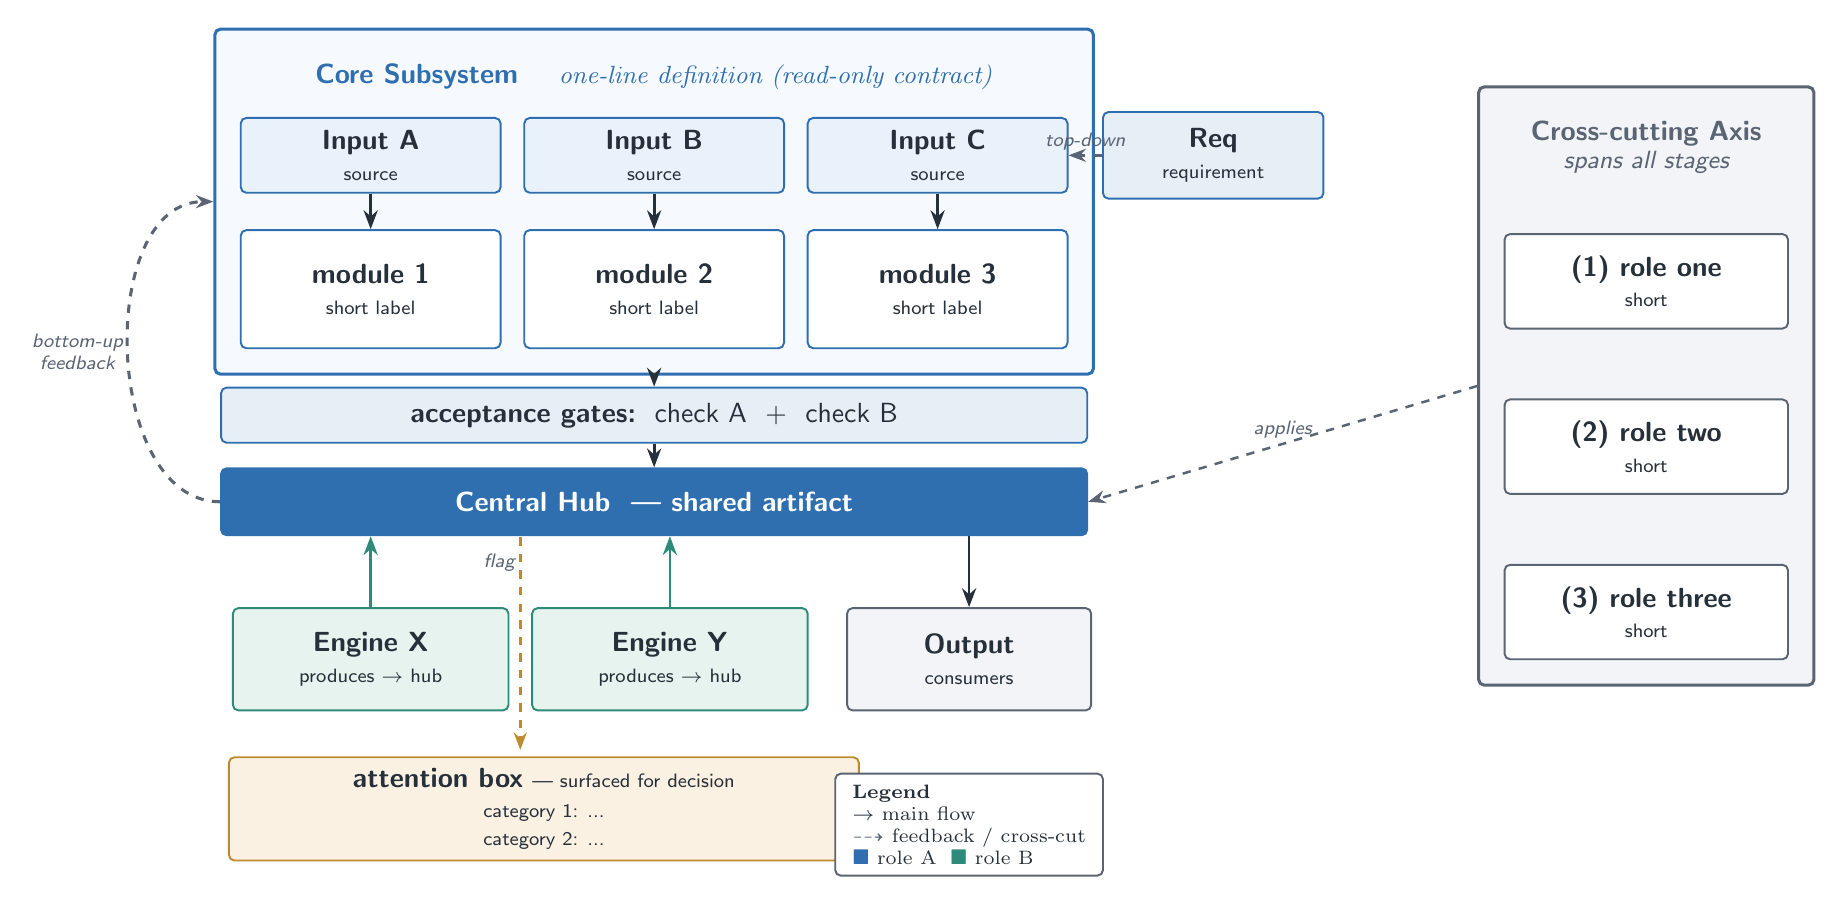
\begin{tikzpicture}[
  font=\sffamily, >=Stealth,
  box/.style={rounded corners=2pt, draw, line width=0.7pt, align=center, inner sep=4pt, text=ink},
  mod/.style={box, fill=white, draw=coreline, minimum width=3.3cm, minimum height=1.5cm},
  inp/.style={box, fill=corefill, draw=coreline, minimum width=3.3cm, minimum height=0.95cm},
  engine/.style={box, fill=datafill, draw=dataline, minimum width=3.5cm, minimum height=1.3cm},
  output/.style={box, fill=railfill, draw=railline, minimum width=3.1cm, minimum height=1.3cm},
  warn/.style={box, fill=warnfill, draw=warnline, minimum width=8cm, minimum height=1.3cm},
  role/.style={box, fill=white, draw=railline, minimum width=3.6cm, minimum height=1.2cm},
  bar/.style={box, fill=hubfill, draw=hubfill, text=white, minimum width=11cm, minimum height=0.85cm, font=\sffamily\bfseries},
  gate/.style={box, fill=hubfill!12, draw=hubfill, minimum width=11cm, minimum height=0.7cm},
  flow/.style={-{Stealth[length=2.4mm]}, line width=1pt, draw=ink},
  dflow/.style={-{Stealth[length=2.4mm]}, line width=1pt, draw=dataline},
  feed/.style={-{Stealth[length=2.2mm]}, line width=0.9pt, draw=railline, dashed},
  lbl/.style={font=\sffamily\scriptsize\itshape, text=railline, inner sep=1.5pt},
]

% ===== CORE subsystem (inputs row -> modules row), wrapped in a fit container =====
\node[inp] (i1) at (2.2,10.2) {\textbf{Input A}\\[-1pt]{\scriptsize source}};
\node[inp] (i2) at (5.8,10.2) {\textbf{Input B}\\[-1pt]{\scriptsize source}};
\node[inp] (i3) at (9.4,10.2) {\textbf{Input C}\\[-1pt]{\scriptsize source}};
\node[mod] (m1) at (2.2,8.5)  {\textbf{module 1}\\[-1pt]{\scriptsize short label}};
\node[mod] (m2) at (5.8,8.5)  {\textbf{module 2}\\[-1pt]{\scriptsize short label}};
\node[mod] (m3) at (9.4,8.5)  {\textbf{module 3}\\[-1pt]{\scriptsize short label}};
\node[font=\sffamily\bfseries, text=coreline] (ctitle) at (5.8,11.2)
  {Core Subsystem \quad\textnormal{\small\mdseries\itshape one-line definition (read-only contract)}};
\begin{scope}[on background layer]
  \node[box, fill=corefill!40, draw=coreline, line width=1.1pt,
        fit=(ctitle)(i1)(i2)(i3)(m1)(m2)(m3), inner sep=9pt] (core) {};
\end{scope}
\draw[flow] (i1)--(m1);  \draw[flow] (i2)--(m2);  \draw[flow] (i3)--(m3);

% external requirement feeding a module (top-down)
\node[box, fill=hubfill!12, draw=hubfill, minimum width=2.8cm, minimum height=1.1cm] (req) at (12.9,10.2)
  {\textbf{Req}\\[-1pt]{\scriptsize requirement}};
\draw[feed] (req) -- node[lbl,above]{top-down} (m3.east|-req);

% ===== gate + hub =====
\node[gate] (gate) at (5.8,6.9) {\textbf{acceptance gates:}\ \ check A\ \ $+$\ \ check B};
\node[bar]  (hub)  at (5.8,5.8) {Central Hub \ —\ shared artifact};
\draw[flow] (core.south)--(gate.north);
\draw[flow] (gate.south)--(hub.north);

% ===== engines + output =====
\node[engine] (e1)  at (2.2,3.8) {\textbf{Engine X}\\[-1pt]{\scriptsize produces $\to$ hub}};
\node[engine] (e2)  at (6.0,3.8) {\textbf{Engine Y}\\[-1pt]{\scriptsize produces $\to$ hub}};
\node[output] (o1)  at (9.8,3.8) {\textbf{Output}\\[-1pt]{\scriptsize consumers}};
\draw[dflow] (e1.north)--(e1.north|-hub.south);
\draw[dflow] (e2.north)--(e2.north|-hub.south);
\draw[flow]  (hub.south-|o1.north)--(o1.north);

% ===== attention / limbo box =====
\node[warn] (pend) at (4.4,1.9)
  {\textbf{attention box}\ {\scriptsize— surfaced for decision}\\[-1pt]
   {\scriptsize category 1: ...}\\[-2pt]{\scriptsize category 2: ...}};
\draw[feed, draw=warnline] (4.1,5.35)--(4.1,2.65) node[lbl,pos=0.12,left]{flag};

% ===== bottom-up feedback on the left margin (curve, no crossings) =====
\draw[feed, line width=1.1pt] (hub.west) to[out=180,in=180]
  node[lbl,left,align=center,pos=0.5]{bottom-up\\feedback} (core.west);

% ===== side rail (cross-cutting axis) =====
\node[role] (r1) at (18.4,8.6) {\textbf{(1) role one}\\[-1pt]{\scriptsize short}};
\node[role] (r2) at (18.4,6.5) {\textbf{(2) role two}\\[-1pt]{\scriptsize short}};
\node[role] (r3) at (18.4,4.4) {\textbf{(3) role three}\\[-1pt]{\scriptsize short}};
\node[font=\sffamily\bfseries, text=railline, align=center] (rtitle) at (18.4,10.3)
  {Cross-cutting Axis\\[-2pt]{\small\mdseries\itshape spans all stages}};
\begin{scope}[on background layer]
  \node[box, fill=railfill, draw=railline, line width=1.1pt,
        fit=(rtitle)(r1)(r2)(r3), inner sep=9pt] (rail) {};
\end{scope}
\draw[feed] (rail.west)-- node[lbl,above]{applies} (hub.east);

% ===== legend =====
\node[box, fill=white, draw=railline, align=left, font=\scriptsize, text=ink,
      minimum width=3.4cm] at (9.8,1.7)
  {\textbf{Legend}\\
   \textcolor{ink}{$\rightarrow$} main flow\\
   \textcolor{railline}{$\dashrightarrow$} feedback / cross-cut\\
   \textcolor{coreline}{$\blacksquare$} role A \;\textcolor{dataline}{$\blacksquare$} role B};

\end{tikzpicture}
\end{document}
